\chapter{Autotuning Symbolic Optimization\\Fabrics for Trajectory Generation}
\label{cha:icra_23}

%% The following annotation is customary for chapter which have already been
%% published as a paper.
\blfootnote{Parts of this chapter have been published in  \cite{Spahn2023}.}
\blfootnote{
  This chapter is a mere copy of the work presented at \acl{icra} 2023 in
  London, UK, \cite{Spahn2023}. The background section has been removed to
  avoid repetition from \cref{cha:background}.
}

%% It is only necessary to list the authors if multiple people contributed
%% significantly to the chapter.
%\authors{Max Spahn, Javier Alonso-Mora}

\begin{abstract}
In the previous chapter, we have defined \ac{tg} as the problem of finding a
sequence of actions that will move the robot from its current state to a
desired state. As this thesis focuses on \ac{tg} for mobile manipulation,
relevant literature must therefore include works from different fields, ranging
from autonomous driving and mobile robotics to manipulation. Besides, \ac{tg} in
dynamic environments generally includes path planning and local \ac{tg}.
Therefore, this chapter summarizes approaches ordered on a scale of reactivity,
that is the frequency at which trajectories are computed. Starting with
controller-like \ac{tg} methods, we then move in order of increasing
time-horizon up until global path planning. At last, we
recall environmental representations for \ac{tg}.
\end{abstract}


\newpage

%%%%%%%%%%%%%%%%%%%%%%%%%%%%%%%%%%%%%%%%%%%%%%%%%%%%%%%%%%%%%%%%%%%%%%%%%%%%%%%%

\section{Introduction}
\label{sec:intro}


As robots are making their way into human shared environments,
fast reactive behavior is needed to make sure that obstacles are safely avoided
at all time. Trajectory optimization methods, such as Model Predictive Control,
are widely used to guarantee collision avoidance during execution. While such
methods perform well in slowly changing environments, their computational costs
limit the achievable computation frequencies cannot be considered truly reactive. 
\ac{fabrics} offer an
alternative to classic trajectory optimization techniques. Based on differential
geometry, policies are composed of several components to form a highly reactive
and fast behavior. However, the composition of \ac{fabrics} of
individual obstacle avoidance geometries is limited to simple geometric shapes,
such that a differentiable distance function can easily be formulated. The 
sets a challenging requirement on the perception part of the motion generation
pipeline. In this work, we present and analyse three different methods to 
overcome this drawback, namely integration of \ac{fsd}, 
\acp{sdf} and raw sensor data into the framework of
\ac{fabrics}. While putting more computational effort onto the fabrics planner, it
relaxes the computational costs of the perception pipeline.
In the process, we derive essential extensions to the framework and
analyse strength and weaknesses of the individual methods. To summarize, this
paper makes the following contributions:
\begin{itemize}
  \item We integrate implicit representation of the environment into the
    framework of \ac{fabrics}, namely \ac{fsd}, \ac{sdf}
    and raw sensor data.
  \item We derive how numerical gradients can be used for pullback operations
    which are essential in the composition of \ac{fabrics}.
  \item We analyse strength and weaknesses of the three representations in
    dynamic environments.
  \item We present real-world experiments illustrating the power of our
    open-source implementation.
\end{itemize}

\section{Environment representations}
\label{sec:environment_representations}

All above described methods rely on some form of environment
representation. For example, the inequality constraints in
\ac{mpc} formulations responsible for collision avoidance
rely on a distance function between the robot and the
obstacles. Path planning methods, as described above, 
also require an environment representation, such that
collision checking can accept or reject new samples. In
geometric approaches, such as \ac{apf}, \ac{rmp} and
\ac{fabrics}, distance functions are also necessary.
For primitive shapes, such as spheres and boxes, distances
can be computed in closed form. When working in dynamic
environments, robots perceive their environment using vision
sensors, such as cameras, or range sensors, such as LiDAR.
Classifying the environment into primitive shapes is a
challenging task, especially when the environment is
cluttered and parts are occluded. A different approach to
collision avoidance relies on more implicit representations
of the environments --the most implicit would be raw sensor
data. In the following, we recall some works that focus on
such representations in the context of \ac{tg}.

\subsection{Implicit representations}
\label{sub:implicit_representations}

For trajectory planning using short-term optimization,
unoccupied space constraints limit robot movement, proven
useful for mobile robots in cluttered areas
\cite{Brito2019}. In drone flight, a similar concept
generates safe flight zones along a global path
\cite{Liu2017a,Tordesillas2019a,tordesillas2021mader}. In
the context of drone flying, \ac{sdf} has been utilized with
\ac{mpc} trajectory generation in unknown environments
\cite{Oleynikova2017voxblox}. Raw Lidar data has been used
in combination with \acp{rmp} showing impressively high
frequencies when computation is parallelized on GPU
\cite{Pantic2023obstacle}. Recent advances in sampling-based
\ac{mpc}, utilizing physics engines for collision avoidance
\cite{Pezzato2023sampling}, integrate obstacle collisions in
cost functions during trajectory rollouts. A similar
approach is seen in \cite{Sundaralingam2023curobo}. For
these approaches, the environment representation is implicit
through integration into the cost function, but requires
accurate modeling of the robot and the environment in the
physics engine used for rollout computation.

Though many methods demand manual robot representation, like
composing spheres, exploration of even more implicit
characterizations, such as learned \ac{sdf} like in
\cite{Liu2022regularized,Koptev2023neural}, is underway.

\begin{figure}
  \centering
  \input{src/24-spahn-ral/img/methods/inkscape/spectrum_tex.pdf_tex}
  \caption{Different levels of implicitness for environment representations.}
  \label{fig:overview}
\end{figure}




\section{Related Work}

Robotic mobile manipulation stands as a dynamic and expansive field of research, spurred by diverse potential applications and further fueled by prestigious
international competitions, such as DARPA’s Robotics Challenge
\cite{darpa_challenge}, RoboCup@Home~\cite{robocup_home}, the Amazon Picking
Challenge \cite{corbato2018integrating}, and RoboCup@Work \cite{robocup_work}. These
competitions are tailored to address distinct challenges and performance
criteria. Numerous research projects have yielded a significant number of
various mobile manipulation platforms. For an exhaustive overview of wheeled
mobile manipulation systems and the associated challenges, readers can refer to
\cite{overview1,overview2}. 

A supermarket mobile manipulator showcase has been presented in \cite{toyota2023} with a special focus on metrics in real-world settings and the importance of quantitative field experiments. Similar long-term fetch and carry experiments, yet in different environments, were carried out by Domel et al.~\cite{domel2017toward} in a factory environment and by Stibinger et al.~\cite{vstibinger2021mobile} in an outdoor competition to pick up and place simulated
construction materials. Instead of relying on a  Model Predictive Control formulation, such as presented in ~\cite{minniti2021model} for motion planning and control, we deploy a more reactive trajectory generation method \cite{ratliff2023fabrics}, and a task planning and execution approach that is more adaptive in the presence of disturbances.





\section{Overview}
\label{sec:overview}
%
In this paper, we first recall very briefly the theory of optimization fabrics and the steps
to use it for trajectory generation (\cref{sec:optimization_fabrics}). Then, we formulate 
optimization fabrics as a symbolic trajectory generator, so that combining
of individual components is only performed once (\cref{sec:symbolic_fabrics}).
Then, we formulate parameter tuning for trajectory generation as a constrained optimization problem
and propose Bayesian optimization for effective autotuning (\cref{sec:tuning}).  
As an example, we apply this autotuning to symbolic optimization
fabrics (\cref{sec:icra23_experimental_results}), but it is generally 
independent of the trajectory generator at hand.


%\section{Background}
\label{sec:math}
%
We introduce some notations and the mathematical operations 
from differential geometry used in the framework of
\ac{fabrics}. This introduction is rather limited and the
reader is referred to \cite{Ratliff2021,Spahn2023,Wyk2022} for a more in-depth
introduction.
%
\subsection{Configurations and task variables}%
\label{sub:configurations_and_task_variables}
%
We denote $\q\in\Q\subset\Rn$ a configuration of the robot with $n$ its degrees
of freedom; \Q{} is the configuration space of the generalized coordinates of
the system. Generally, $\q(t)$ defines the robot's configuration at time $t$, so
that \qdot, \qddot{} define the instantaneous derivatives of the robot's
configuration. Similarly, we assume that there is a set of task variables
$\xj\in\Xj\subset\Rmj$ with variable dimension $m_j \leq n$. The task space
\Xj{} defines an arbitrary manifold of the configuration space \Q{} in which a
robotic task can be represented. Further, we assume that there is a differential
map $\map_j:\Rn\rightarrow\Rmj$ that relates the configuration space to the
$j^{th}$ task space. For example, when a task variable is defined as the
end-effector position, then $\map_j$ is the positional part of the forward
kinematics. On the other hand, if a task variable is defined to be the joint
position, then $\map_j$ is the identity function. In the following, we drop the
subscript $j$ in most cases for readability when the context is clear.

We assume that \map{} is in $\mathcal{C}^1$ so that the Jacobian is
defined as
\begin{equation}
  \J = \derf{\q}{\map} \in \mathcal{R}^{m\times n}, 
\end{equation}
or $\J = \der{\q}{\map}$ for short.
Thus, we can write the total time derivatives of \x{} as
$\xdot = \J\qdot$ and $\xddot = \J\qddot + \Jdot\qdot$.
%
\subsection{Spectral semi-sprays}%
\label{sub:semi_spectral_sprays}
%
The framework of
\ac{fabrics} designs trajectory generation as second-order dynamical systems $\xddot =
\pi(\x,\xdot)$~\cite{Cheng2020,Ratliff2020}. The trajectory is defined by the
differential equation $\M\xddot + \f = 0$, where $\M(\x,\xdot)$ and
$\f(\x,\xdot)$ are functions of position and velocity. Besides, \M{} is
symmetric and invertible. We denote such systems as $\Spec = \spec$ and refer to
them as \textit{spectral semi-sprays}, or \textit{specs} for
short. Often, we drop the subscript $\X$ when the context is clear.
%
\subsection{Operations on specs}%
\label{sub:operations_on_specs}
%
Trajectory generation requires the combination of multiple
components, such as collision avoidance, joint limits
avoidance, etc.
In the framework of \ac{fabrics}, these components are
represented as specs in different manifolds and combined in a consistent way using
a metric-weighted sum.
Related operations from differential geometry are recalled
here.

Given a differential map $\map: \Q\rightarrow\X$ and a spec \spec{}, the \textit{pullback}
is defined as 
\begin{equation}
  \pull{\map}{\spec} = {\left(\Jt\M\J, \Jt(\f+\Jdot\qdot)\right)}_{Q}.
  \label{eq:pullback}
\end{equation}
The pullback allows converting between two distinct manifolds (e.g. a spec could be 
defined in the robot's workspace and pulled into the robot's configuration space using
the pullback with \map{} being the forward kinematics).

For two specs, $\Spec_1 = {\left(\M_1,\f_1\right)}_{\X}$ and 
$\Spec_2 = {\left(\M_2,\f_2\right)}_{\X}$, their \textit{summation} is defined by:
\begin{equation}
  \Spec_1 + \Spec_2 = {\left(\M_1 + \M_2, \f_1 + \f_2\right)}_{\X}.
  \label{eq:specs_summation}
\end{equation}
%

Additionally, a spec can be \textit{energized} by a Lagrangian energy. Effectively, 
this equips the spec with a metric.
Specifically, given a spec of form $\Spec_{\vec{h}} = (\mat{I},\vec{h})$ and 
an energy Lagrangian \le{} with the derived equations of motion $\M_{\le}\xddot + \f_{\le} =0$, 
we can define the operation
\begin{equation}
  \begin{split}
  S_{\vec{h}}^{\le} &= \text{energize}_{\le}\{S_{\vec{h}}\} \\
    &= (\Me, \fe + \Pe[\Me\vec{h} - \fe]), 
  \end{split}
  \label{eq:energization}
\end{equation}
where $\Pe = \Me\left(\Me^{-1} - \frac{\xdot\xdot^T}{\xdot^T\Me\xdot}\right)$ is an
orthogonal projector. The resulting spec is an \textit{energized spec} and 
we call the operation \textit{energization}.

With spectral semi-sprays and the presented operations,
avoidance behavior, such as joint limit avoidance, collision
avoidance or self-collision avoidance, can be realized.

\subsection{Optimization fabrics}%
\label{sub:optimization_fabrics}
%
In the previous subsection, we recalled how different avoidance behaviors can
be combined. Spectral semi-sprays can additionally be \textit{forced} by a
potential, denoted as the \textit{forced variant} of form $\Spec_{\forc} =
\left(\M,\f + \der{\x}{\forc}\right)$. This forcing term clearly changes the
behavior of the system. Under certain conditions, it can be
shown that the trajectory $\x(t)$ of the forced variant converges towards the minimum of the potential \forc{}~\cite{Ratliff2020}.

First, the initial spec that represents an avoidance
component is written in the form $\xddot + \vec{h}(\x,\xdot)
= 0$, such that $\vec{h}$ is \textit{homogeneous of degree
2}: $\vec{h}(\x,\alpha\xdot) = \alpha^2\vec{h}(\x,\xdot)$
(\textbf{Creation}). Secondly, the geometry is energized
(\cref{eq:energization}) with a Finsler
structure~\cite[Definition 5.4]{Ratliff2020}
(\textbf{Energization}). The property of homogeneity of
degree 2 and the energization with the Finsler structure
guarantees, according to ~\cite[Theorem 4.29]{Ratliff2020},
that the energized spec forms a \textit{frictionless
fabric}. A frictionless fabric is defined to optimize the
forcing potential \forc{} when being damped by a positive
definite damping term~\cite[Definition 4.4]{Ratliff2020}.
Thirdly, all avoidance components are combined in the
configuration space of the robot using the pullback and
summation operation (\textbf{Combination}). Note, that both
operations are closed under the algebra designed by these
operations, i.e. every pulled optimization fabric or the sum
of two \ac{fabrics} is, itself, an optimization fabric. In
the last step, the combined spec is forced by the potential
\forc{} with the desired minimum and damped with a positive
definite damping term (\textbf{Forcing}). This resulting
system of form $\M\qddot + \f(\q, \qdot) + \der{\q}{\forc} +
\beta\qdot = 0$ is solved to obtain the trajectory
generation policy in acceleration form $\qddot = \pi(\q,\qdot)$.



\section{Derivation of dynamic fabrics}%
\label{sec:methods}

We extend the framework of optimization fabrics to \acf{df}.
including
dynamic environments and path following tasks. We prove that \ac{df}
converge to moving goals and can be combined with previous approaches in geometric
control.
%
This section first introduces the notion of reference trajectory, dynamic Lagrangians and
the dynamic pullback. These notations allow then to formulate \ac{df}. 
As \ac{df} generalize the concept of optimization fabrics to dynamic scenarios, we refer 
to the non-dynamic fabrics as \acf{sf} to explicitly distinguish between the work
presented in \cite{Ratliff2020} and our work.

\subsection{Motion design using dynamic fabrics}%
\label{sub:motion_design_using_dynamic_fabrics}

The method explained in this paper generalizes the concept of \ac{sf}
from \cite{Ratliff2020} and can then be extended from the procedure outlined in \cref{sub:trajectory_generation_using_optimization_fabrics}.

\begin{enumerate}
  \item Design path-consistent geometries in a suited, \textbf{time-parameterized} (\cref{def:dynamic_map}) manifold of the configuration
  \item Design corresponding Finsler energies defining the importance metric in this manifold.
  \item Energize all geometries with the associated Finsler energies.
  \item \textbf{If necessary, pull back the energized system from the time-parameterized manifold into
    the corresponding fixed manifold (\cref{eq:dynamic_pull})}.
  \item Pull back the energized system into the configuration space and combine it with
    all components using summation.
  \item Force the system with a \textbf{time-parameterized} potential. As a composition of \ac{df}, 
    the resulting trajectory converges towards the potential's minimum (\cref{lem:dynamic_lagrangian_fabrics}).
\end{enumerate}
In the following, we explain our proposed changes to the framework of \ac{sf} so that it remains
valid in dynamic environments.

\subsection{Reference trajectories}%
\label{sub:reference_trajectories}

To enable the definition of dynamic convergence and dynamic energy we introduce
a reference trajectory that remains inside a domain \X{} as \textit{boundary conforming}.
This term is chosen in accordance to \cite[Definition 4.6]{Ratliff2020}.
\begin{definition}
  A reference trajectory $\xt(t)$, with its corresponding time derivatives \xtdot{} and
  \xtddot{}, is boundary conforming on the manifold \X{} if $\xt(t) \in \X, \forall t$.%
  \label{def:refTraj}
\end{definition}

In the following, the reference trajectory will be used to define 
dynamic Lagrangians and dynamic fabrics. In this context, the word `dynamic' can often
be read as `relative to the reference trajectory'.
With the notion of reference trajectories we formulate a mapping to the relative
coordinate system.
\begin{definition}
  Given a reference trajectory \xt{} on \X{}, the dynamic mapping
  $\mapd : \X\times\X \to \Xr$ represents the relative coordinate system
  $\xr = \x - \xt$. 
  \label{def:dynamic_map}
\end{definition}

\begin{figure}[h]
  \centering
  \begin{subfigure}{0.5\linewidth}
    \centering
    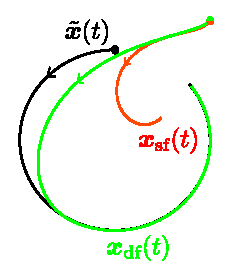
\includegraphics[height=\textwidth]{methods/reference_trajectory}
    \caption{Dynamic convergence}%
    \label{subfig:reference_trajectory_1}
  \end{subfigure}%
  \begin{subfigure}{0.5\linewidth}
    \centering
    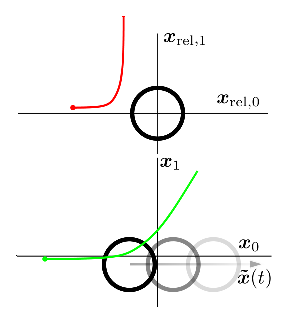
\includegraphics[height=\textwidth]{methods/reference_pull_no_equations}
    \caption{Dynamic Avoidance}%
    \label{subfig:reference_trajectory_2}
  \end{subfigure}
  \caption{The two implications of \acl{df}. 
    In (a), it can be seen that the trajectory obtained with \ac{df} (green)
    converges towards the reference trajectory (black) while the trajectory
    with \acl{sf} (red) does not converge. 
    In (b), the top part
    visualizes collision avoidance as suggested in~\cite{Ratliff2020}. Here,
    the trajectory and obstacle are expressed
    in a relative system $\xr$. Using the dynamic pull, \cref{eq:dynamic_pull}, this
    can be transformed into the static reference frame $\x$, bottom part. Together
    with dynamic energization, the framework of optimization fabrics is leveraged
    for dynamic environments.
    The motion of the obstacle, $\xr(t)$ is visualized with an arrow, future positions
    of the obstacle are shown in lighter color. The resulting trajectory obtained with
    \ac{df} is shown in green.
  }%
  \label{fig:reference_trajectory}
\end{figure}

\subsection{Dynamic pullback}%
\label{sub:dynamic_pullback}

%Specs can be formulated with the relative coordinate \xr{}, as described in
%\cite{Ratliff2020}. 
%The theory remains valid with relative coordinates when all components
%are defined in the same relative coordinates.
The theory of optimization fabrics also applies to relative coordinates \xr{}, specifically,
specs and potentials can be formulated in moving coordinates. However, 
there is no theory to combine specs defined in relative coordinates with specs in fixed
coordinates.
In most cases, individual components of the
behavior design are not formulated in the same relative coordinates. Specificially, the
configuration space is always static, so we introduce a transformation of a relative spec
into the static space \X{}. We call this operation \textit{dynamic pullback}.
\begin{equation}
  \pull{\mapd}{{(\Md,\fd)}_{\Xr}} = {(\Md, \fd - \Md\xtddot)}_{\X}
  \label{eq:dynamic_pull}
\end{equation}
Two specs $\Spec_{\X_{\textrm{rel,1}}}$ and $\Spec_{\X_{\textrm{rel,2}}}$ defined
in two different relative coordinate systems are then combined by
first applying the dynamic pullback to both individually and then applying the summation
operation for specs. The dynamic pullback is the natural extension to optimization fabrics
for relative coordinate systems. It cannot directly be
integrated into the framework of optimization
fabrics as it breaks the algebra. In the following, we derive several
generalizations so that the theory remains 
valid even in the presence of reference trajectories for individual components, such as moving
obstacles or reference trajectories.

\subsection{Dynamic Lagrangians}%
\label{sub:dynamic_lagrangians}

Next, we show that energy conservation commutes with the dynamic pullback. This allows us to
transfer findings on conservative fabrics to dynamic fabrics.
We call a Lagrangian that is defined using relative coordinates
a \textit{dynamic Lagrangian} and write $\ld(\xr, \xrdot)$. 
In this relative coordinate system, the dynamic
Lagrangian has the same properties as the Lagrangian defined in~\cite{Ratliff2020},
specifically it induces the Lagrangian spec through the Euler-Lagrange equation, 
$\dertwo{\xrdot\xrdot}{\ld}\xrddot + \dertwo{\xrdot\xr}{\ld}\xrdot - \der{\xr}{\ld}$, 
as $(\Mde,\fde)$. The system's Hamiltonian $\hd = \der{\xrdot}{\ld}^T\xrdot - \ld$ is
conserved by the equation of motion as proven in~\cite{Ratliff2020}.

Applying the dynamic pullback to the dynamic Lagrangian we obtain the transformed
Lagrangian $\ld(\x, \xdot, \xt, \xdot)$ in the static coordinate system.

\begin{theorem}
  Let $\ld(\xr,\xrdot)$ be a dynamic Lagrangian and let \mapd{} be
  the dynamic mapping to \xr{}. Then, the application of the Euler-Lagrange equation
  commutes with the dynamic pullback.
  \label{the:dynamic_euler_lagrange}
\end{theorem}

\begin{proof}
  We will show the equivalence by calculation. As shown above, the induced spec is defined
in the relative system as $(\Mde, \fde)$. It can be dynamically pulled to form
\begin{equation}
  \pull{\mapd}{{(\Mde,\fde)}_{\Xr}} = {(\Mde, \fde - \Mde\xtddot)}_{\X}
  \label{eq:proof_theorem_euler_commutes}
\end{equation}
We can dynamically pull the Lagrangian $\ld(\xr,\xrdot)$
to form $\ld(\x,\xdot,\xt,\xtdot)$, where only the first two variables are system
variables. Using the generalized Euler-Lagrange equation, the equations of motion of the
pulled Lagrangian are obtained as
\begin{align*}
  0 &= \dert{\derf{\xdot}{\ld}}
      - \derf{\x}{\ld} \\
    &=  \derftwo{\xdot}{\xdot}{\ld}\xddot
      + \derftwo{\xdot}{\x}{\ld}\xdot
      + \derftwo{\xdot}{\xtdot}{\ld}\xtddot
      + \derftwo{\xdot}{\xt}{\ld}\xtdot
      - \derf{\x}{\ld} \\
    &=  \derftwo{\xrdot}{\xrdot}{\ld}\derf{\xdot}{\xrdot}\derf{\xdot}{\xrdot}\xddot 
      + \derftwo{\xrdot}{\xr}{\ld}\derf{\xdot}{\xrdot}\derf{\x}{\xr}\xdot \\
      &+ \derftwo{\xrdot}{\xrdot}{\ld}\derf{\xdot}{\xrdot}\derf{\xtdot}{\xrdot}\xtddot
      + \derftwo{\xrdot}{\xr}{\ld}\derf{\xdot}{\xrdot}\derf{\xt}{\xr}\xtdot \\
      &- \derf{\xr}{\ld}\derf{\x}{\xr} \\
    &=  \derftwo{\xrdot}{\xrdot}{\ld}\xddot
      + \derftwo{\xrdot}{\xr}{\ld}\xdot
      - \derftwo{\xrdot}{\xrdot}{\ld}\xtddot \\
      &- \derftwo{\xrdot}{\xr}{\ld}\xtdot
      - \derf{\xr}{\ld} \\
    &=  \derftwo{\xrdot}{\xrdot}{\ld}(\xddot - \xtddot)
      + \derftwo{\xrdot}{\xr}{\ld}(\xdot - \xtdot)
      - \derf{\xr}{\ld} \\
    &=  \derftwo{\xrdot}{\xrdot}{\ld}(\xddot - \xtddot)
      + \derftwo{\xrdot}{\xr}{\ld}(\xrdot)
      - \der{\xr}{\ld} \\
    &= \Mde \xddot + \fde - \Mde\xtddot
\end{align*}
The obtained equations of motion match the one obtained by applying the dynamic pullback,
see \cref{eq:proof_theorem_euler_commutes}.
\end{proof}
Hence, independently of the coordinates, the system conserves the energy \hd{} computed with the
Hamiltonion in relative coordinates.
Next, we adapt the operation of energization to dynamic Lagrangians. 
Dynamic Lagrangians are a necessary step to allow
for collision avoidance with dynamic obstacles in the framework of
optimization fabrics.
Specifically, the metric for a moving obstacle is computed
using the Euler-Lagrange equation in the relative coordinate system. Importantly, 
in this system, the same energies as with \ac{sf} can be employed. Using the dynamic
pullback, the energy defining the metric for the moving obstacle is then maintained
according to \cref{the:dynamic_euler_lagrange}. Concretely, this means that
collision avoidance can be achieved in a similar manner as with \ac{sf} with the added
advantage of integrated motion estimates of obstacles.

\begin{proposition}[Dynamic Energization]
  Let ${\xddot + \vec{h}(\x,\xdot) = \vec{0}}$ be a differential equation and suppose \ld{} is a
dynamic Lagrangian with the induced spec $(\Mde,\fde)$ and dynamic energy \hd{}. Then the
dynamically energized system~{$\xddot + \vec{h}(\x,\xdot) + \alpha_{\hd}\xrdot = \vec{0}$} with 
\[
  \alpha_{\hd} = -{(\xrdot^T\Mde\xrdot)}^{-1}\xrdot^T(\Mde(\vec{h}+\xtddot)-\fde)
\]
conserves the dynamic energy \hd{}.%
\label{prop:dynamic_energization}
\end{proposition}
\begin{proof}
  From the derivations in~\cite{Ratliff2020}, we can compute the rate of change of the
dynamic energy as $\dot{\hd} = \xrdot^T(\Mde\xrddot + \fde)$. The equations of motion can be
plugged in through the definition of the reference trajectory \cref{def:refTraj}, 
$\xrddot = \xddot - \xtddot$ to obtain:
\begin{align*}
  \dot{\hd} &= \xrdot^T(\Mde(-\vec{h}-\alpha_{\hd}\xrdot - \xtddot) + \fde) \\
  &= \xrdot^T(-\Mde\vec{h}-\Mde\xrdot\alpha_{\hd} - \Mde\xtddot + \fde) \\
  &= \xrdot^T(-\Mde\vec{h} \\
      & +\Mde\xrdot{(\xrdot^T\Mde\xrdot)}^{-1}\xrdot^T(\Mde(\vec{h}+\xtddot)-\fde) \\
      & - \Mde\xtddot + \fde) \\
  &= -\xrdot^T\Mde\vec{h}
      +\xrdot^T(\Mde(\vec{h}+\xtddot)-\fde) \\
      & - \xrdot^T\Mde\xtddot + \xrdot^T\fde \\
  &= 0
\end{align*}
The energized system conserves the dynamic energy.
\end{proof}
\cref{prop:dynamic_energization} allows to combine dynamic components of the
motion generator
with static components. Effectively, the dynamic component \textit{bends} the
underlying geometry according to the motion of the dynamic components (e.g., a moving
obstacle).

While dynamic Lagrangians and the corresponding energization operation are similar to the
methods described in~\cite{Ratliff2020}, the operation of the standard pull to the
dynamically energized system must be slightly modified. Specifically, the reference
velocity must be pulled. We show that dynamic
energization also commutes with the standard pullback.

\begin{theorem}
Let \ld{} be a dynamic Lagrangian to the reference trajectory \xt{}, and
let~{$\xddot+\h(\x, \xdot) = \vec{0}$} be a second order differential equation with a metric \Md{}
such that $\Jt\Md\J$ has full rank that can be written as spec $(\Md, \Md\h)$. Suppose $x =
\map(\q)$ is a differential map with \J{} its Jacobian. Then
\begin{equation}
  \energize{\pull{\map}{\ld}}{\left(\pull{\map}{(\I, \h)}\right)} =
\pull{\map}{\left(\energize{\ld}{(\I,\h)}\right)}, 
\end{equation}
when the reference velocity is being pulled as $\qtdot = \pinv{\J}\xtdot$.
$\pinv{\J}$ denotes the pseudo-inverse of \J{}.
%
We say that the dynamic energization operation commutes with the pullback transform.
\end{theorem}
\begin{proof}
  The commutation can be proven by calculation. First, we compute the right side of the
equivalence. According to \cref{prop:dynamic_energization}, the energized system (that
maintains the dynamic energy \hd{}) writes as 
\[
  \Md\xddot + \Md\h + \alpha_{\hd}(\xdot-\xtdot) = 0, 
\]
with $\alpha_{\hd}$ as defined in \cref{prop:dynamic_energization}.
Applying the pull-operation, we obtain
\begin{equation}
  \Jt\Md\J\qddot + \Jt\Md\h + \Jt\Md\Jdot\qdot + \Jt\Md\alpha_{\hd}(\xdot-\xtdot) = 0.
  \label{eq:pulled_energized_system}
\end{equation}
As the equation expressed in \X{}, this equation in \Q{} maintains the energy \hd{}. Next,
we compute the left hand side. The equation of motion of the pulled dynamic Lagrangian \ld{}
computes as 
\begin{align*}
  \pull{\map}{(\Md,\fd)}
    &= \Jt\left(\Md\J\qddot  + \fd + \Md\Jdot\qdot - \Md\xtddot\right)\\
    &= \tilde{\Md}\qddot  + \tilde{\fd} - \Jt\Md\xtddot.
\end{align*}
The original spec is pulled accordingly
\begin{align*}
  \pull{\map}{(\Md,\Md\h)} &=
  \Jt\Md\J\qddot + \Jt\Md\h + \Jt\Md\Jdot\qdot \\
  &= \tilde{\Md}\qddot + \tilde{\Md}\tilde{\h}
\end{align*}
We energize the pulled system according to \cref{prop:dynamic_energization}
\begin{equation}
  \begin{split}
    \Jt\Md\J\qddot + \Jt\Md\h + \Jt\Md\Jdot\qdot \\
    + \Jt\Md\J\alpha_{\pull{\map}{\hd}}(\qdot-\pinv{\J}\xdot) = 0, 
  \end{split}
\label{eq:energized_pulled_system}
\end{equation}
with 
\begin{align*}
  \alpha_{\pull{\map}{\hd}} = 
    & -{\left({(\qdot-\pinv{\J}\xtdot)}^T\Jt\Md\J(\qdot-\pinv{\J}\xtdot)\right)}^{-1} \\
    & {(\qdot-\pinv{\J}\xtdot)}^T\left(\Jt\Md\J(\tilde{\h}+\xtddot)\right. \\
    & - \left.\Jt\fd - \Jt\Md\Jdot\qdot\right) \\
    = & -{\left({(\J\qdot-\J\pinv{\J}\xtdot)}^T\Md(\J\qdot-\J\pinv{\J}\xtdot)\right)}^{-1} \\
    & {(\qdot-\pinv{\J}\xtdot)}^T\left(\Jt\Md\J\tilde{\h}+\Jt\Md\xtddot\right. \\
    & \left.- \Jt\fd - \Jt\Md\Jdot\qdot\right) \\
    = & -{\left({(\xdot-\xtdot)}^T\Md(\xdot-\xtdot)\right)}^{-1} \\
    & {(\qdot-\pinv{\J}\xtdot)}^T\left(\Jt\Md\h + \Jt\Md\Jdot\qdot +\Jt\Md\xtddot\right. \\
    & \left.- \Jt\fd - \Jt\Md\Jdot\qdot\right) \\
    = & -{\left({(\xdot-\xtdot)}^T\Md(\xdot-\xtdot)\right)}^{-1} \\
    & {(\qdot-\pinv{\J}\xtdot)}^T\left(\Jt\Md\h + \Jt\Md\xtddot- \Jt\fd \right) \\
    = & -{\left({(\xdot-\xtdot)}^T\Md(\xdot-\xtdot)\right)}^{-1} \\
    & {(\J\qdot-\J\pinv{\J}\xtdot)}^T\left(\Md\h + \Md\xtddot- \fd \right) \\
    = & -{\left({(\xdot-\xtdot)}^T\Md(\xdot-\xtdot)\right)}^{-1}
    {(\xdot-\xtdot)}^T\\
    & \left(\Md\h + \Md\xtddot- \fd \right) \\
    & = \alpha_{\hd}
\end{align*}
Thus, we have shown equivalence between $\alpha_{\hd}$
and $\alpha_{\pull{\map}{\hd}}$. As $\alpha$ is scalar we can can rewrite the energization
term in \cref{eq:energized_pulled_system} as
\begin{align*}
  &\Jt\Md\J\alpha_{\pull{\map}{\hd}}(\qdot-\pinv{\J}\xdot)\\
  = &\Jt\Md\alpha_{\pull{\map}{\hd}}(\J\qdot-\J\pinv{\J}\xdot)\\
  = &\Jt\Md\alpha_{\pull{\map}{\hd}}(\xdot-\xdot)\\
  = &\Jt\Md\alpha_{\hd}(\xdot-\xdot)\\
\end{align*}
With the equivalence of the energization terms, we conclude the
proof that dynamic energization commutes with the standard pullback.
\end{proof}

\subsection{Dynamic fabrics}%
\label{sub:dynamic_fabrics}

With the previous results, we formulate a new class of fabrics that converge to a
reference trajectory. We call this class of fabrics \acl{df}. 
First, some notations are introduced to eventually show that dynamically energized specs
form dynamic fabrics.
%
\iffalse%
\begin{definition}
A spec is called \textit{dynamically converging} towards a reference $\xt(t)$,
if and only if
\[
  \exists t_1 \geq 0, \forall t \geq t_1:
      \xddot(t) = \xtddot(t), \xdot(t) = \xtdot(t), \x(t) = \xt(t),
\]
For clarity, we say that the spec is dynamically converging with respect to $\xt$, or
dynamically converging for short if the reference is clear from the context.
\end{definition}
\fi
%
Analogously to unbiased specs, we define dynamically unbiased specs (i.e., specs whose
solutions do not diverge from the reference \xt{} when starting on the reference).
\begin{definition}
A spec is said to be \textit{dynamically unbiased} with respect to $\xt(t)$ if
$\f(\x, \xdot) = -\M\xtddot$, for $\x(t) = \xt(t)$ and $\xdot(t) = \xtdot(t)$.
\end{definition}

Beside being dynamically unbiased, some specs will converge to the reference trajectory
independently from their initial conditions.

\begin{definition}
A spec is \textit{dynamically rough} with respect to $\xt(t)$ if all
its integral curves $\x(t)$ converge dynamically with respect to $\xt(t)$.
\end{definition}

As for \ac{sf}, \ac{df} can be formed by
specs when they are being forced by a potential function \forc. Such a forcing potential is
generally a function of \x{} and \xt{} and has at least one minimum. A spec that converges
to a minimum of the forcing potential then forms a dynamic fabrics.

\begin{definition}
A spec forms a \textit{dynamically rough fabric} if it is dynamically rough with respect
to $\xt(t)$ when forced by a dynamic potential and 
$\exists t_1 > 0$ such that $\forall t>t_1, \x(t)$ satisfies the
Karush-Kuhn-Tucker (KKT) conditions for the optimization problem $\text{min}_{\x\in\X} \forc(\x,
\xt(t))$. If a spec does not form a dynamically rough fabric but all its damped variants
do, it forms a \textit{dynamically frictionless fabric}.
\end{definition}

\begin{theorem}[Dynamic Fabrics]
%Suppose $S=(\M,\f)_{\X}$ is a dynamic spec with respect to \xt{}.
Suppose $S={(\M,\f)}_{\X}$ is a spec.  Then $S$ forms a dynamically rough fabric with
respect to \xt{} if and only if it is dynamically unbiased with respect to \xt{} and it
converges dynamically when being forced by a dynamic potential $\forc(\x,\xt)$ with
$\norm{\der{\x}{\forc}} < \infty$ on \X{}.%
\label{the:dynamic_fabrics}
\end{theorem}

\begin{proof}
We can write the corresponding differential equation
\begin{equation}
  \M\xddot + \f = -\der{\x}{\forc}
  \label{eq:proof_4_10_b}
\end{equation}
Assume that $S$ is dynamically unbiased.
Since the spec converges with respect to $\xt(t)$, we have $\xdot\to\xtdot, \x\to\xt$.
Because it is dynamically unbiased we also have $\f\to-\M\xtddot$.
Thus, the left hand side of
\cref{eq:proof_4_10_b}, approaches $\vec{0}$.
Consequently, the right hand side must also
approach $\vec{0}$ and hence $\der{\x}{\forc} \to \vec{0}$. The last satisfies the 
Karush–Kuhn–Tucker (KKT)
conditions of \forc{}.

To prove the converse, assume \f{} dynamically biased. That implies that 
\[
  \exists t > 0, \f = \M\xtddot + \vec{a}(\xt, \xtdot),
    \vec{a}(\xt, \xtdot) \neq \vec{0}.
\]
Hence, there exist a $t > 0$ for which the left hand side does not vanish. As \forc{}
satisifies the KKT conditions at $\x = \xt$, its derivative equals zero at $\x = \xt$ which contradicts
\cref{eq:proof_4_10_b} with $\M\vec{a}(\xt, \xtdot) = \vec{0}$.
\end{proof}

Hence, the spec is required to be unbiased and convergent when forced. While the former
can be verified using straight-forward computation, convergence is difficult to verify in
the general case. 

% \MS{Are we sure that dynamically energized specs are dynamically unbiased?}
\begin{lemma}[Dynamically energized fabrics]
  Suppose $S$ is a dynamically unbiased energized spec. Then $S$
  forms a dynamically frictionless
  fabric if  $\der{\x}{\forc} = -\der{\xt}{\forc}$.%
\label{lem:dynamically_energized_fabrics}
\end{lemma}
\begin{proof}
  The equation of motion for the energized, forced and damped system writes as 
  \begin{equation}
    \xddot + \vec{h} + \alpha_{\hd}\xrdot + \mat{B}\xrdot + \der{\x}{\forc} = 0
  \end{equation}
  The systems energy (dynamic Hamiltonian) is used as a Lyapunov function to show
  convergence. The rate of change is computed as
  \begin{align*}
    \dot{\hd^{\forc}} &= \xrdot^T(
      \Mde(
        -\vec{h}
        - \alpha_{\hd}\xrdot 
        - \mat{B}\xrdot 
        - \der{\x}{\forc}
        - \xtddot) \\
      & + \fde) 
      + \dot{\forc} \\
              &= -\xrdot^T\mat{B}\xrdot
      - \xrdot^T\der{\x}{\forc}
      + \xdot^T\der{\x}{\forc}
      + \xtdot^T\der{\xt}{\forc} \\
              &= -\xrdot^T\mat{B}\xrdot \\
  \end{align*}

  As the system energy is lower bounded with $\hd + \forc \geq 0$ and 
  $\dot{\hd^{\forc}} \leq 0$, when $\mat{B}$ stricly positive definite, we must have
$\dot{\hd^{\forc}} \to 0$. Thus, \xrdot{} goes to zero. We can conclude that the system is
dynamically converging. As it it also said to be dynamically unbiased, the damped
energized system forms a dynamic fabric by \cref{the:dynamic_fabrics}.
\end{proof}

\begin{lemma}[Dynamic Lagrangian fabrics]
An unbiased, dynamic Lagrangian spec forms a dynamically frictionless
fabric if  $\der{\x}{\forc} = -\der{\xt}{\forc}$ holds for the forcing term.
\label{lem:dynamic_lagrangian_fabrics}
\end{lemma}
\begin{proof}
The equations of motion induced by the dynamic Lagrangian including damping and forcing 
are defined by the spec and can
be written explicitly as
\begin{align}
  \M_{\ld}\xrddot + \f_{\ld} + \mat{B}\xrdot + \der{\x}{\forc} = 0 \nonumber \\
  \M_{\ld}(\xddot - \xtddot) + \f_{\ld} + \mat{B}(\xdot - \xtdot) + \der{\x}{\forc} = 0
\label{eq:motion} \\
  \M_{\ld}\xddot - \M_{\ld}\xtddot + \f_{\ld} + \mat{B}\xdot - \mat{B}\xtdot +
    \der{\x}{\forc} = 0 \nonumber
\end{align}

In the following we use the Hamiltonian and the potential function as Lyapunov function to
show convergence of the damped spec.
\begin{align*}
  \hd^{\forc}(\x) &= \hd + \forc \\
  &= \der{\xrdot}{\ld^T}\xrdot - \ld + \forc
\end{align*}
The time derivative is composed of the time derivative of the Hamiltonian, $\dot{\he} =
\xrdot^T (\M_{\ld}\xrddot + \f_{\ld})$, and the time derivative of the forcing potential, 
$\dot{\forc} = \xdot^T\der{\x}{\forc} + \xtdot^T\der{\xt}{\forc}$.
Thus, the system's total energy varies over time:
\[
  \dot{\hd}^{\forc}(\x) = {(\xdot - \xtdot)}^T(\M_{\ld} (\xddot - \xtddot) + \f_{\ld}) +
\xdot^T\der{\x}{\forc} + \xtdot^T\der{\xt}{\forc}
\]
Plugging in the equations of motion \cref{eq:motion} gives
\begin{align*}
  \dot{\hd}^{\forc}(\x) &= {(\xdot - \xtdot)}^T(-\f_{\ld} - \mat{B}(\xdot - \xtdot) - \der{\x}{\forc} +
    \f_{\ld}) \\
  &  + \xdot^T\der{\x}{\forc} + \xtdot^T\der{\xt}{\forc} \\
  &= -{(\xdot - \xtdot)}^T\mat{B}(\xdot - \xtdot) - {(\xdot - \xtdot)}^T\der{\x}{\forc} \\
  & + \xdot^T\der{\x}{\forc} + \xtdot^T\der{\xt}{\forc} \\
  &= -{(\xdot - \xtdot)}^T\mat{B}(\xdot - \xtdot)
    + \xtdot^T(\der{\x}{\forc} + \der{\xt}{\forc}).
\end{align*}
For $\der{\x}{\forc} = -\der{\xt}{\forc}$ and $\mat{B}$ strictly positive definite,
$\dot{\hd}$ is strictly negative for $(\xdot - \xtdot) \neq 0$. Since $\hd^{\forc}$ is lower
bounded as composition of lower bounded function and $\dot{\hd}^{\forc} \leq 0$,
$\dot{\hd}^{\forc} \to 0$ and thus, $\xdot \to \xtdot$ and $\x \to \xt$. Hence, the spec
converges dynamically with respect to \xt{}.
As the spec is further said to be
dynamically unbiased, the damped spec forms a dynamic fabric by \cref{the:dynamic_fabrics}.
\end{proof}

Concretely, \cref{lem:dynamic_lagrangian_fabrics} allows for trajectory following
with guaranteed convergence with \ac{df}. For example, a reference trajectory 
for the robot's end-effector is defined as $\xt(t)$. Then, the potential can be designed
as $\psi = \xt(t) - \x$ (respecting the construction rule required
for \cref{lem:dynamic_lagrangian_fabrics}). In contrast to \ac{sf}, where the static
potential function is simply updated at every time step, \ac{df} makes use of the dynamics 
of the reference trajectory through the dynamic pullback.

\subsection{Construction procedure}

From the high-level procedure explained in \cref{sub:motion_design_using_dynamic_fabrics}, we can
derive the algorithm using the formal findings in this section, see \cref{alg:motion_design}.
\begin{algorithm}
  Define basic inertia as spec $\M\qddot + \M\h = 0$ \\
  \For{avoidance in avoidances}{
    Define differential map between \Q{} and $\X_i$: $\map$ or $\map_t$ \\
    Design geometry on $\X_i$: $\xddot_i + \h_{2,i} = \zerovec$ \\
    Design Finsler energy for behavior on $\X_i$: $\l_i$ \\
    Energize geometry with Finsler energy \ref{prop:dynamic_energization}\\
    \If{\map{} is time-parameterized}{
      Apply dynamic pullback to energized system\\
    }
    Apply standard pullback\\
    Add pulled avoidance component to root fabric\\
  }
  Force root system with (time-parameterized) potential\\
  \caption{Motion design with dynamic fabrics}
  \label{alg:motion_design}
\end{algorithm}

Methods to design the individual components, such as geometry and 
Finsler structures, are introduced in~\cite{Ratliff2020}.
As these design patterns do not vary for \ac{df}, they are not repeated here.
In the result section, we show some experimental examples highlighting
the comparative advantage of
optimization fabrics over model predictive schemes and the advantage of \ac{df}
over \ac{sf} for dynamic environments.



\section{Experimental Results}
\label{experimental_results}

The presented method is evaluated in simulation and with the real hardware. After a short introduction to the experimental setup, three simulation scenarios and one real-world scenario are introduced. We compare the presented method with a sequenced MPC formulation in which arm motion and locomotion are sequenced and a conventional MPC formulation in which inequalities are formulated for individual obstacles. Scenarios are considered infeasible when following the trajectory without global replanning is not possible without violating the collision constraints.
%
\subsection{Experimental Setup}%
\label{sub:experimental_setup}

\paragraph{Hardware Setup}
The mobile manipulator used to validate this approach consists of the mobile base \textit{Clearpath\textsuperscript{TM} Boxer} and the robotic manipulator \textit{Franka Emika Panda}, see ~{Fig. \ref{fig:real_robot}}. The
resulting system has 10 \acp{dof} for which
the dynamics are approximated using a Runge-Kutta scheme to
obtain the discrete transition function $f(\z_t, \u_t)$.
The presented robot is equipped with low level controllers that accept commanded velocities
for all joints, one LiDAR sensor  and one
depth camera pointing forward. Laser data and camera depth images are fused into one
pointcloud using the octomap framework \cite{Hornung2013}. Polyhedrons to describe the
convex space around the links are computed using the \textit{DecompUtil} presented in
\cite{Liu2017}, into which the pointcloud generated from the vertex centers of the
occupied cells of the octomap are fed.
Joint positions for the arm are known at every time step using the encoders and the pose
of the base is estimated using SLAM.
The implementation is realized in the \textit{Robotics Operating System} (ROS) framework, as it
allows simple integration of the different components. The underlying MPC
problem is solved using \textit{FORCES-Pro} solver \cite{forcespro} and employing an interior-point method\cite{FORCESNLP}. We used a laptop with an Intel Core i7 and 32GB of RAM to run the simulations and an Intel NUC with an Intel Core i7 and 8GB to run the real-world experiments.

\paragraph{Parameter Details}%
\label{par:parameter_details}
%
The presented robot has nine links which are represented by four spheres for collision avoidance. The positions of the spheres on the kinematic chain are explicitly given in Table
\ref{tab:spheres}. Note that the robot is not fully contained in the union of spheres. For
$d_{\textrm{safety}} = 0$, this could potentially result in collision. However, much
larger spheres would result in the inability to move close to obstacles when manipulation
is requested. The parametrization with $d_{\textrm{safety}}$ allows to flexibly change
between different motion types, e.g. manipulation (low safety margin) and navigation
(large safety margin). The centers of the given spheres are also used as seed points
for the convex region
generation. Two different step size were used over the time horizon, $\Delta t_1, \Delta t_2$. All remaining parameter settings are summarized in Table
\ref{tab:parameters}. 
%
\begin{table}[!t]
  \centering
  \caption{Positions of spheres for the volumetric representation.}
  \label{tab:spheres}
  \begin{tabular}{|c|c|c|}
    \hline
    Parent Link & Offset & Radius \\
    \hline
    base link & [0, 0, 0.25] & 0.25 \\
    \hline
    base link & [0.3, 0, 0.25] & 0.25 \\
    \hline
    link 2 & [0, -0.1896, 0] & 0.2275 \\
    \hline
    link 7 & [0, 0, 0] & 0.3 \\
    \hline
  \end{tabular}
\end{table}
%
\begin{table}[h]
  \centering
  \caption{Parameter Settings}
  \label{tab:parameters}
  \begin{tabular}{|c|c|c|}
  \hline
  Parameter & Static Scenarios & Dynamic Scenario\\
  \hline
  Prediction Horizon & $11$ sec & $11s$ sec\\
  \hline
  $\Delta t_1$/$\Delta t_2$ & $0.2$/$1.0$ sec & $0.2$/$1.0$ sec\\
  \hline
  \#Planes/Link & $15$ & $15$ \\
  \hline
  $d_{\textrm{safety}}$ & $0.15$ m & $0.25$ m \\
  \hline
  $W_{\vec{e}}$ & $5.0\mat{I}_2$ & $5.0\mat{I}_2$\\
  \hline
  $w_{\theta}$ & $2.0$ & $2.0$\\
  \hline
  $W_\vq$ & $0.7 \mat{I}_7$ & $0.7 \mat{I}_7$ \\
  \hline
  $W_\vu$ & $\begin{bmatrix} 0.05\mat{I}_2 & 0 \\ 0 & 5\mat{I}_7 \end{bmatrix}$ &
  $\begin{bmatrix} 0.05\mat{I}_2 & 0 \\ 0 & 5\mat{I}_7 \end{bmatrix}$ \\
  \hline
  $w_{\textrm{slack}}$ & $10^{5}$ & $10^{5}$\\
  \hline
  \end{tabular}
\end{table}
%
%
\subsection{Manipulation Scenarios}%
\label{sub:environment_setup}

We compare our proposed method against two baseline methods: a decoupled MPC baseline (i.e., locomotion and arm motion are performed sequentially) and a coupled MPC formulation based on sphere-sphere inequality constraints, as proposed in \cite{Avanzini2018}. Moreover, as this work presents a method for local trajectory optimization, the effect of global replanning during the execution is not considered. To access our method's performance, we present simulation results for:
\begin{itemize}
    \item Static collision avoidance with a horizontal bar \cite{Avanzini2018} (Sub-section \ref{par:horizantal_bar});
    \item 2D trajectory tracking while avoiding collisions with randomly placed static obstacles (Sub-section \ref{par:randomized_obstacles});
    \item Dynamic collision avoidance with a moving obstacle (Sub-section \ref{par:dynamic_obstacle}).
\end{itemize} 
Finally, we present experimental results on a mobile manipulator performing a real manipulation task (Sub-section \ref{par:real_world}).

\paragraph{Horizontal Bar}
\label{par:horizantal_bar}
%
A horizontal bar is placed between the start and goal configuration. In contrast to the work in \cite{Avanzini2018}, no object detection is required in our approach, as the sensed point cloud is fed directly into the convex region generator. The base's global path consists of a simple straight-line motion to a pose behind the bar. The motion of the manipulator and the generated convex regions for the last link of the kinematic chain are depicted in ~{Fig. \ref{fig:bar_motion}}. 
% Improved flexibility
The advantage of whole-body optimization can be extracted when the horizontal bar is placed at a lower $z$-positions. In ~{Fig. \ref{fig:feasibility_issue}}, such a situation is visualized for $z=1.3$. In the visualized case, it is not possible to move underneath the bar with the sequenced approach. On the other hand, the coupled method can navigate safely avoiding collision by moving the arm into an extended position in which the absolute height is smaller than when having it folded.
%
\begin{figure}[h]
    \centering
    \begin{subfigure}[b]{0.45\linewidth}
        \includegraphics[width=0.9\textwidth]{bar/adv_coupling.png}
        \caption{coupled}
    \end{subfigure}
    \begin{subfigure}[b]{0.425\linewidth}
        \includegraphics[width=0.9\textwidth]{bar/adv_decoupling.png}
        \caption{decoupled}
    \end{subfigure}
    \caption{Advantage of coupled MPC when moving underneath a horizontal bar (orange). }
    \label{fig:feasibility_issue}
\end{figure}
%
\begin{figure}[h]
  \centering
  \begin{subfigure}[b]{0.32\linewidth}
    \includegraphics[width=1.0\textwidth]{bar/sequence_pic1.png}
    \caption{$t=0sec$}
  \end{subfigure}
  \begin{subfigure}[b]{0.32\linewidth}
    \includegraphics[width=1.0\textwidth]{bar/sequence_pic2.png}
    \caption{$t=6sec$}
  \end{subfigure}
  \begin{subfigure}[b]{0.32\linewidth}
    \includegraphics[width=1.0\textwidth]{bar/sequence_pic3.png}
    \caption{$t=17sec$}
  \end{subfigure}
  \begin{subfigure}[b]{0.32\linewidth}
    \includegraphics[width=1.0\textwidth]{bar/sequence_pic4.png}
    \caption{$t=25sec$}
  \end{subfigure}
  \begin{subfigure}[b]{0.32\linewidth}
    \includegraphics[width=1.0\textwidth]{bar/sequence_pic5.png}
    \caption{$t=32sec$}
  \end{subfigure}
  \begin{subfigure}[b]{0.32\linewidth}
    \includegraphics[width=1.0\textwidth]{bar/sequence_pic6.png}
    \caption{$t=42sec$}
  \end{subfigure}
  \caption{Avoiding an horizontal bar. The convex region
for the last link of the kinematic chain.}%
  \label{fig:bar_motion}
\end{figure}

%
\paragraph{Randomized Obstacles}%
\label{par:randomized_obstacles}
%
In this scenario, the robot is placed in an unstructured environment with several static obstacles. A global path for the base to reach the goal is computed, but the path is blocked with randomly
generated obstacles, uniformly distributed on the intervals $x \in [2m, 5m], y \in [-2m, 2m], z
\in [0m, 2m]$. Only those obstacles visible to the LiDAR sensors are available for the global planner which generates a path in the 2D plane for the base's motion. Among the randomly generated cases, only those that are feasible for an MPC trajectory optimizer are considered. Two examples for infeasible cases are depicted in ~{Fig. \ref{fig:infeasible}}.

\begin{figure}[!t]
    \centering
    \begin{subfigure}[b]{0.48\linewidth}
        \includegraphics[height=0.9\linewidth]{randObst/infeasible1.png}
    \end{subfigure}
    \begin{subfigure}[b]{0.48\linewidth}
        \includegraphics[height=0.9\linewidth]{randObst/infeasible2.png}
    \end{subfigure}
    \caption{Example for infeasible cases, that were excluded from the test set in randomized scenario.}
    \label{fig:infeasible}
\end{figure}
%
\begin{figure}[t]
  \centering
  \includegraphics[width=0.8\linewidth]{randObst/trajectory.png}
  \caption{Five obstacles avoidance, final configuration in red, occupied voxels in the octomap are represented in orange.}%
  \label{fig:case_2_example}
\end{figure}
%
\begin{figure}[h]
  \centering
  \begin{subfigure}[b]{0.45\linewidth}
    \includegraphics[height=0.7\linewidth]{randObst/increase_solverTimes_spheres.png}
    \caption{Obstacles as spheres}
  \end{subfigure}
  \begin{subfigure}[b]{0.45\linewidth}
    \includegraphics[height=0.7\linewidth]{randObst/increase_solverTimes_convex.png}
    \caption{Convex regions}
  \end{subfigure}
  \caption{Comparison solver performance for an increasing number of obstacles.}%
  \label{fig:randObst_solver}
\end{figure}
\begin{table}
    \centering
    \begin{tabular}{|c|c|c|}
        \hline
         & decoupled & coupled \\
         \hline
         mean & 219.65s & 113.822s \\
         std. deviation & 24.21s & 8.35s\\
         min & 199.27s & 106.83s \\
         max & 270.25s & 131.24s \\
         \hline
    \end{tabular}
    \caption{Compared execution times coupled and decoupled approach for cases that were feasible for both methods.}
    \label{tab:randObst}
\end{table}
%

A successful trajectory of the coupled MPC planner is depicted in ~{Fig. \ref{fig:case_2_example}}. A key advantage of our method is that when the environment is densely populated with obstacles, the solving times are not affected when using convex regions to represent the free space, see Fig. \ref{fig:randObst_solver}. Explicitly formulating sphere-sphere inequality constraints results in an increase of solving time as the environment becomes more densely populated with obstacles. Note that convex region generation becomes only beneficial as the number of obstacles exceeds a critical value, in this case, for 50 obstacles.
Furthermore, parallelizing the locomotion and arm motion allows to reduce the mean overall operational time by 48\%, see ~{Table \ref{tab:randObst}}.
%

\paragraph{Dynamic Obstacle}%
\label{par:dynamic_obstacle}

Here, we evaluate dynamic collision avoidance with a single moving obstacle for different obstacle's velocities. As dynamic object detection and velocity estimation are out of the scope of this work, the state of the obstacle is assumed to be known to the robot during the entire process. In Fig. \ref{fig:dynamic_case}, the experiment is visualized. The goal pose (light grey) is to be reached but a moving sphere, conflicting the goal, must be avoided at all time. 
The proposed MPC formulation's reactivity is investigated using the clearing distance $d_{\textrm{clear}} = \min_i{\norm{\vp^{\textrm{dyn}} - \vp_{i}} - r_i - r_d^{\textrm{dyn}}}$ and the distance to target, $d_{\textrm{target}} = \norm{\vec{z}_{\textrm{des}} - \vec{z}}$, where $\vec{z}_{\textrm{des}}$ is composed of the desired base and arm configuration. Different velocities ($\vec{v}_d^{\textrm{dyn}}$) and different heights ($z_{\textrm{obs}}$) of the moving obstacles were investigated. Fig. \ref{fig:dynamic_distances} shows that our approach successfully avoids collision with dynamic obstacles when moving towards the goal. 
%
\begin{figure}[h]
  \centering
%  \includegraphics[width=1.0\linewidth]{dynFig.png}
  \begin{subfigure}[b]{0.4\linewidth}
    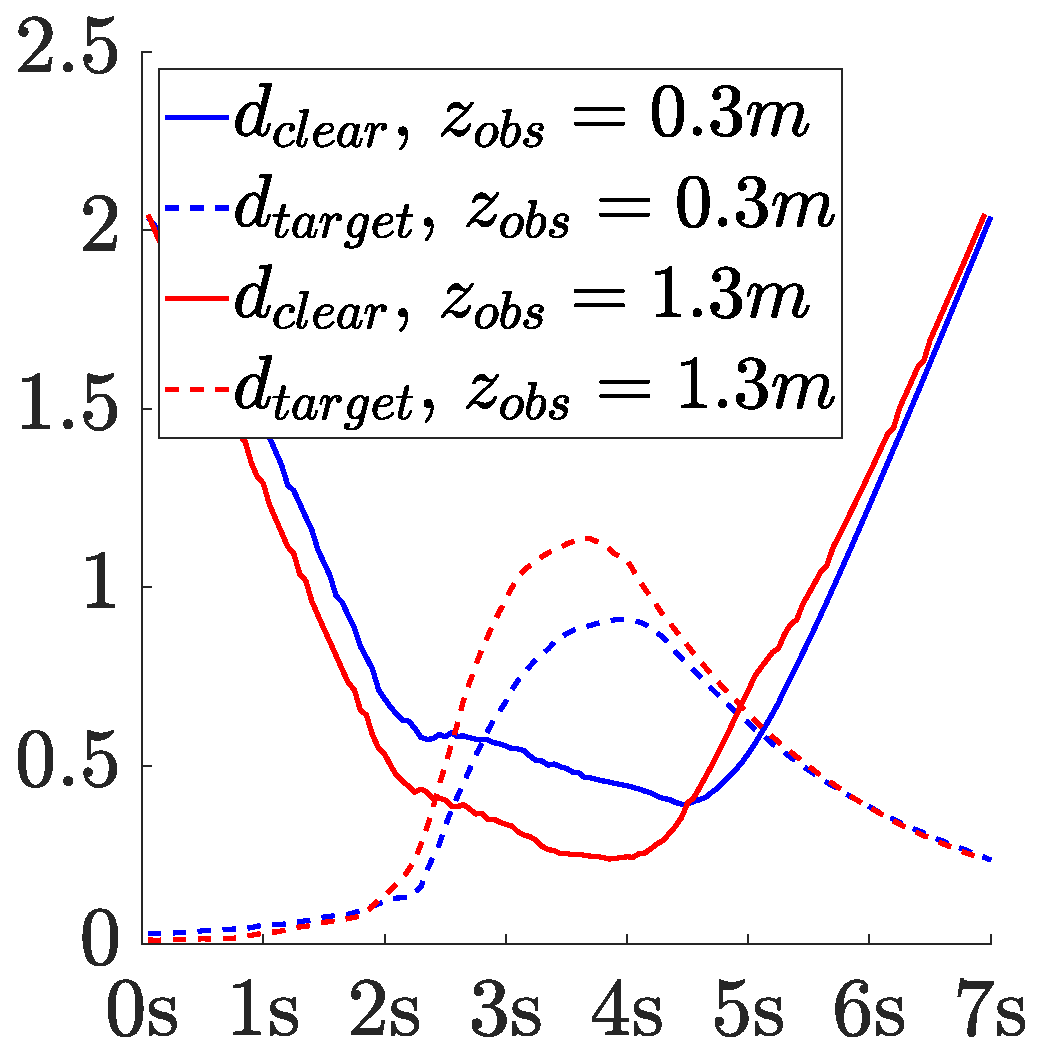
\includegraphics[width=1.0\textwidth]{dynamic/distances_slow}
        \caption{$\norm{\vec{v}_d} = 0.2m/s$}
  \end{subfigure}
  \begin{subfigure}[b]{0.4\linewidth}
    \includegraphics[width=1.0\textwidth]{dynamic/distances_fast}
    \caption{$\norm{\vec{v}_d} = 0.5m/s$}
  \end{subfigure}
  \caption{Clearance from moving obstacle and distance to target position for different obstacle velocities.}%
  \label{fig:dynamic_distances}
\end{figure}
%
\begin{figure}[h]
  \centering
  \begin{subfigure}[b]{0.23\linewidth}
    \includegraphics[width=1.0\textwidth]{dynamic/sequence_pic1.png}
    \caption{$t=0sec$}
  \end{subfigure}
  \begin{subfigure}[b]{0.23\linewidth}
    \includegraphics[width=1.0\textwidth]{dynamic/sequence_pic2.png}
    \caption{$t=1sec$}
  \end{subfigure}
  \begin{subfigure}[b]{0.23\linewidth}
    \includegraphics[width=1.0\textwidth]{dynamic/sequence_pic3.png}
    \caption{$t=2sec$}
  \end{subfigure}
  \begin{subfigure}[b]{0.23\linewidth}
    \includegraphics[width=1.0\textwidth]{dynamic/sequence_pic4.png}
    \caption{$t=3sec$}
  \end{subfigure}
  \caption{Motion avoiding moving obstacle (red) while attempting to reach target (light grey).}%
  \label{fig:dynamic_case}
\end{figure}
%
\paragraph{Real-World Experiment}
\label{par:real_world}
%
\begin{figure}[ht]
  \centering
  \begin{subfigure}[b]{0.23\linewidth}
    \includegraphics[width=1.0\textwidth]{real/sequence_pic1.png}
  \end{subfigure}
  \begin{subfigure}[b]{0.23\linewidth}
    \includegraphics[width=1.0\textwidth]{real/sequence_pic2.png}
  \end{subfigure}
  \begin{subfigure}[b]{0.23\linewidth}
    \includegraphics[width=1.0\textwidth]{real/sequence_pic3.png}
  \end{subfigure}
  \begin{subfigure}[b]{0.23\linewidth}
    \includegraphics[width=1.0\textwidth]{real/sequence_pic4.png}
  \end{subfigure}
  \caption{Trajectory in mock-up store avoiding obstacles, goal configuration in light grey.}%
  \label{fig:real_case}
\end{figure}
%
We evaluated the presented method in real-world scenarios in a simple pick \& place setup. ~{Fig. \ref{fig:real_robot}} depicts the experimental scenario, where the robot picks up an object on the left (pose in light green) and moves to the target pose (pose in light red) without colliding with the obstacle visualized in light blue. Intermediate poses of the successful trajectory are visualized in Fig. \ref{fig:real_case}. A video of the experiment is attached to this work.
%


\chapter{Conclusion and discussion}
\label{cha:conclusion_and_discussion}

The final chapter of this thesis summarizes the contributions and discusses the
main results. Besides, research questions for the following years and raised and
potential approaches are layed out. This chapter ends with a vision on the
future of robotics in human-shared environments.

\section{Conclusion}
\label{sec:conclusion}

This thesis mainly contributed to geometric interpretation of \ac{tg} for manipulators
and mobile manipulators. Specifically, we extended the framework of \ac{fabrics}
to more dynamic environments, proposed a symbolic implementation to allow for
fast parameter tuning at runtime, and demonstrated its effectiveness in
a real demonstration case. Along the way, we showed how \ac{mpc} can be used for
mobile manipulators and why geometric approaches tend to outperform
optimization-based methods for these systems. All results were validate
extensively in simulation and verified in real-world experiments.
In the following, we summarize the main contributions of this thesis.

\section{Discussion}
\label{sec:discussion}






\newpage
